\section{Wasserkraftwerk-Typen}
\subsection{Klassifizierung}
    \vspace{-4mm}
    \def\columnseprulecolor{\color{white}}
    \begin{multicols}{2}
        \begin{itemize}
            \item Laufwasserkraftwerke
            \item Mitteldruckanlagen
            \item Hochdruck- (Speicher-) Anlagen
            \item Pumpspeicherkraftwerke
            \item Gezeitenkraftwerke
            \item Wellenkraftwerke
            \item Wasserwirbelkraftwerke
        \end{itemize}
    \end{multicols}
    \def\columnseprulecolor{\color{black}}

\subsection{Einteilung nach technischen Aspekten}
\vspace{-4mm}
    \def\columnseprulecolor{\color{white}}
    \begin{multicols}{2}
\begin{itemize}
    \item \textbf{Laufwasserkraftwerke}
    \begin{itemize}
        \item Flusskraftwerke
        \begin{itemize}
            \item Blockbauweise
            \item Buchtenkraftwerke
            \item Zwillingsbauweise 
            \item[] (beidseitige Anordnung)
            \item Ausleitkraftwerke
            \item \dots
        \end{itemize}
        \item Ausleitungskraftwerke
    \end{itemize}
    \item \textbf{Speicherkraftwerke} 
    \item[] mit natürlichem Zufluss
    \item \textbf{Pumpspeicherkraftwerke} 
    \item[] (Speicherkraftwerke mit oder ohne natürlichem Zufluss)
    \item Gezeitenkraftwerke
    \item Wellenkraftwerke
\end{itemize}
\end{multicols}
\def\columnseprulecolor{\color{black}}

\subsection{Einteilung nach energiewirtschaftlichen Aspekten}
\begin{itemize}
    \item Grundlastkraftwerke (häufig verwendet, Laufwasser, Speicher mit vielen Volllaststunden)
    \item Mittellastkraftwerke
    \item Spitzenlastkraftwerke (Speicher mit wenig Volllaststunden)
\end{itemize}

\subsection{Einteilung nach Betriebsart}
\begin{itemize}
    \item Verbundbetrieb (im Normalbetrieb alle Kraftwerke in der Schweiz)
    \item Inselbetrieb (Unabhängig vom Netz)
\end{itemize}

\subsection{Einteilung nach der installierten Leistung}
\begin{itemize}
    \item Kleinwasserkraftwerke (in der Regel kleiner 10 MW)
    \item Grosswasserkraftwerke (P > 10 MW)
\end{itemize}

\subsection{Einteilung nach wasserwirtschaftlichen Aspekten}
\begin{itemize}
    \item Wasserkraftwerke, die ausschliesslich elektrische Energie produzieren
    \item Wasserkraftanlagen für mehrere wasserwirtschaftliche Zielsetzungen (Mehrzweckanlagen, z.\,B. Trinkwasser)
\end{itemize}

\subsection{Wasserturbinen und Pumpen}
\begin{itemize}
    \item \textbf{Aktionsturbinen:} Arbeit aus kinetischer Energie-Differenz
    \begin{itemize}
        \item \textbf{Peltonturbinen}
    \end{itemize}
    \item \textbf{Reaktionsturbinen:} Arbeit aus Druckdifferenz vor und nach Turbine
        \begin{itemize}
            \item \textbf{Francisturbinen} (spiralförmig)
            \item \textbf{Kaplanturbinen} (propellerförmig)
            \item Rohrturbinen
            \item Kreiselpumpen als Turbinen
        \end{itemize}
\end{itemize}

\subsection{Laufwasserkraftwerke (LWK)}    
    \begin{minipage}[c]{0.7\columnwidth}
        \begin{center}
            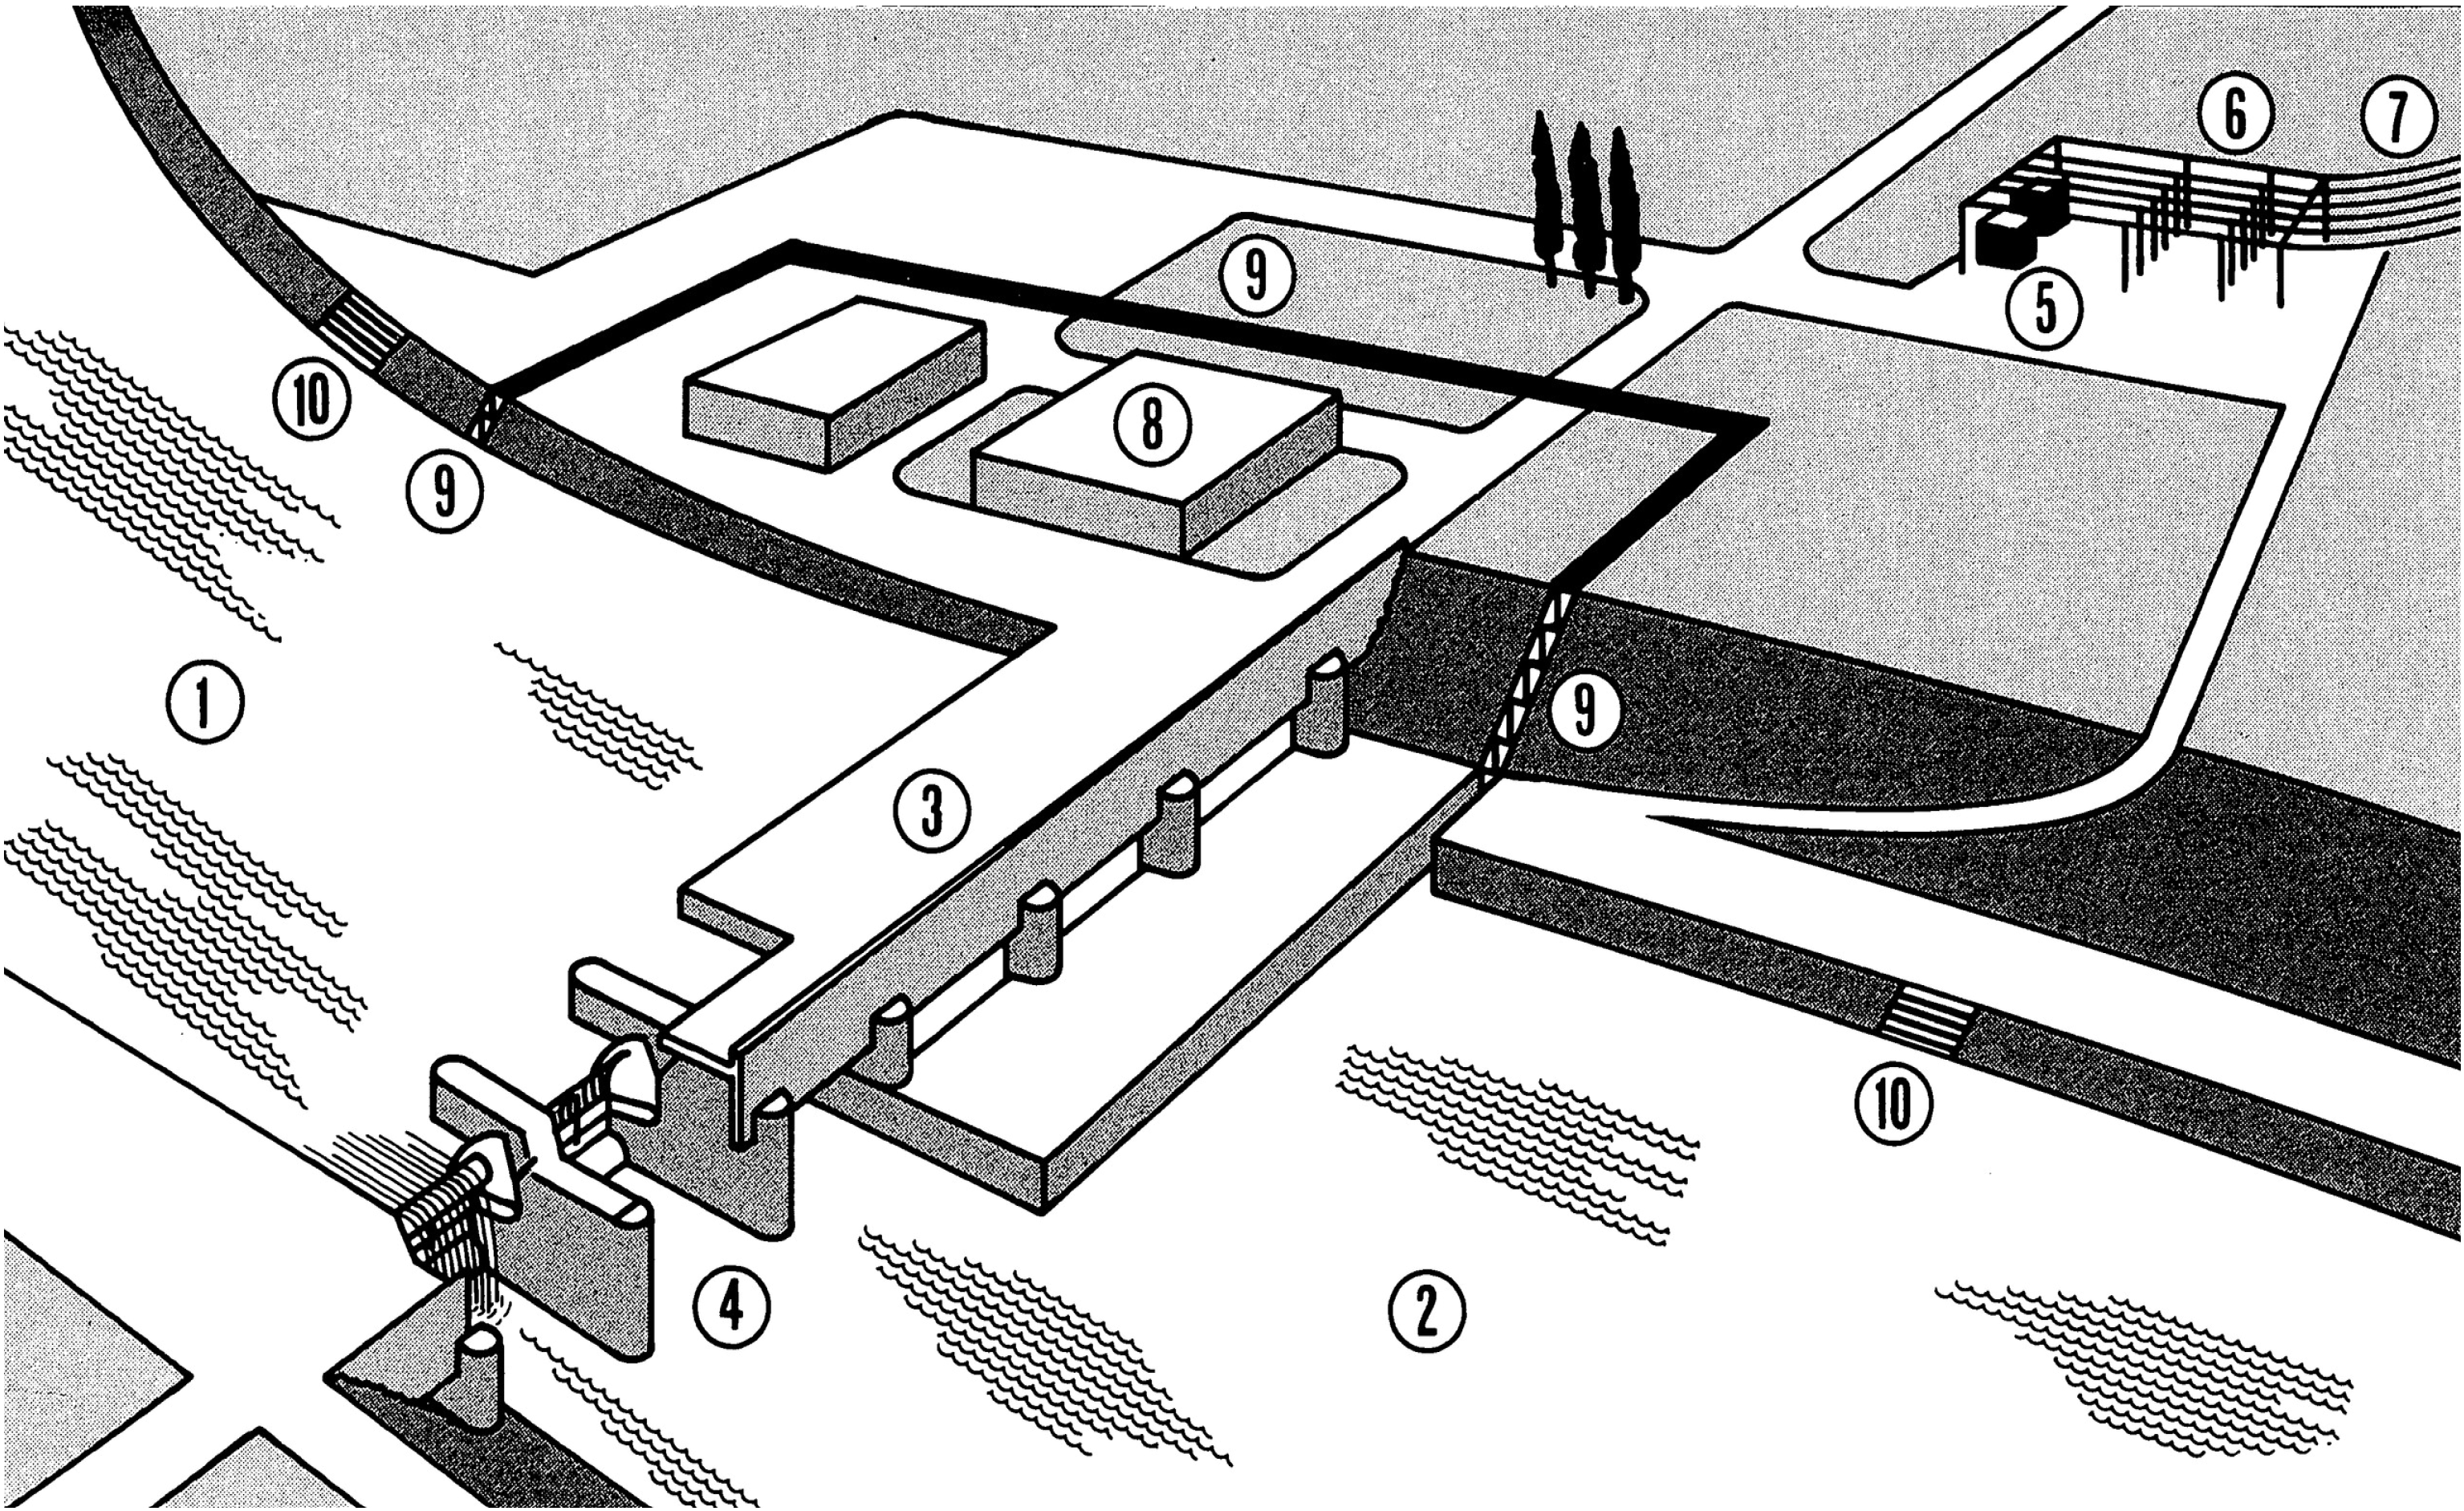
\includegraphics[width=0.95\columnwidth]{images/Laufwasserkraftwerke.png}
        \end{center}
    \end{minipage}
    \hfill
    \begin{minipage}[c]{0.29\columnwidth}
        \begin{enumerate}
            \item Oberwasser 
            \item Unterwasser 
            \item Maschinenhaus
            \item Stauwehr
            \item Transformatoren
            \item Schaltanlage
            \item Leitungen
            \item Betriebsgebäude
            \item Fischtreppe
            \item Einrichtung für den Schiffstransport
        \end{enumerate}
    \end{minipage}

\subsection{LWK mit Kaplanturbinen (vertikal)}
    \begin{center}
        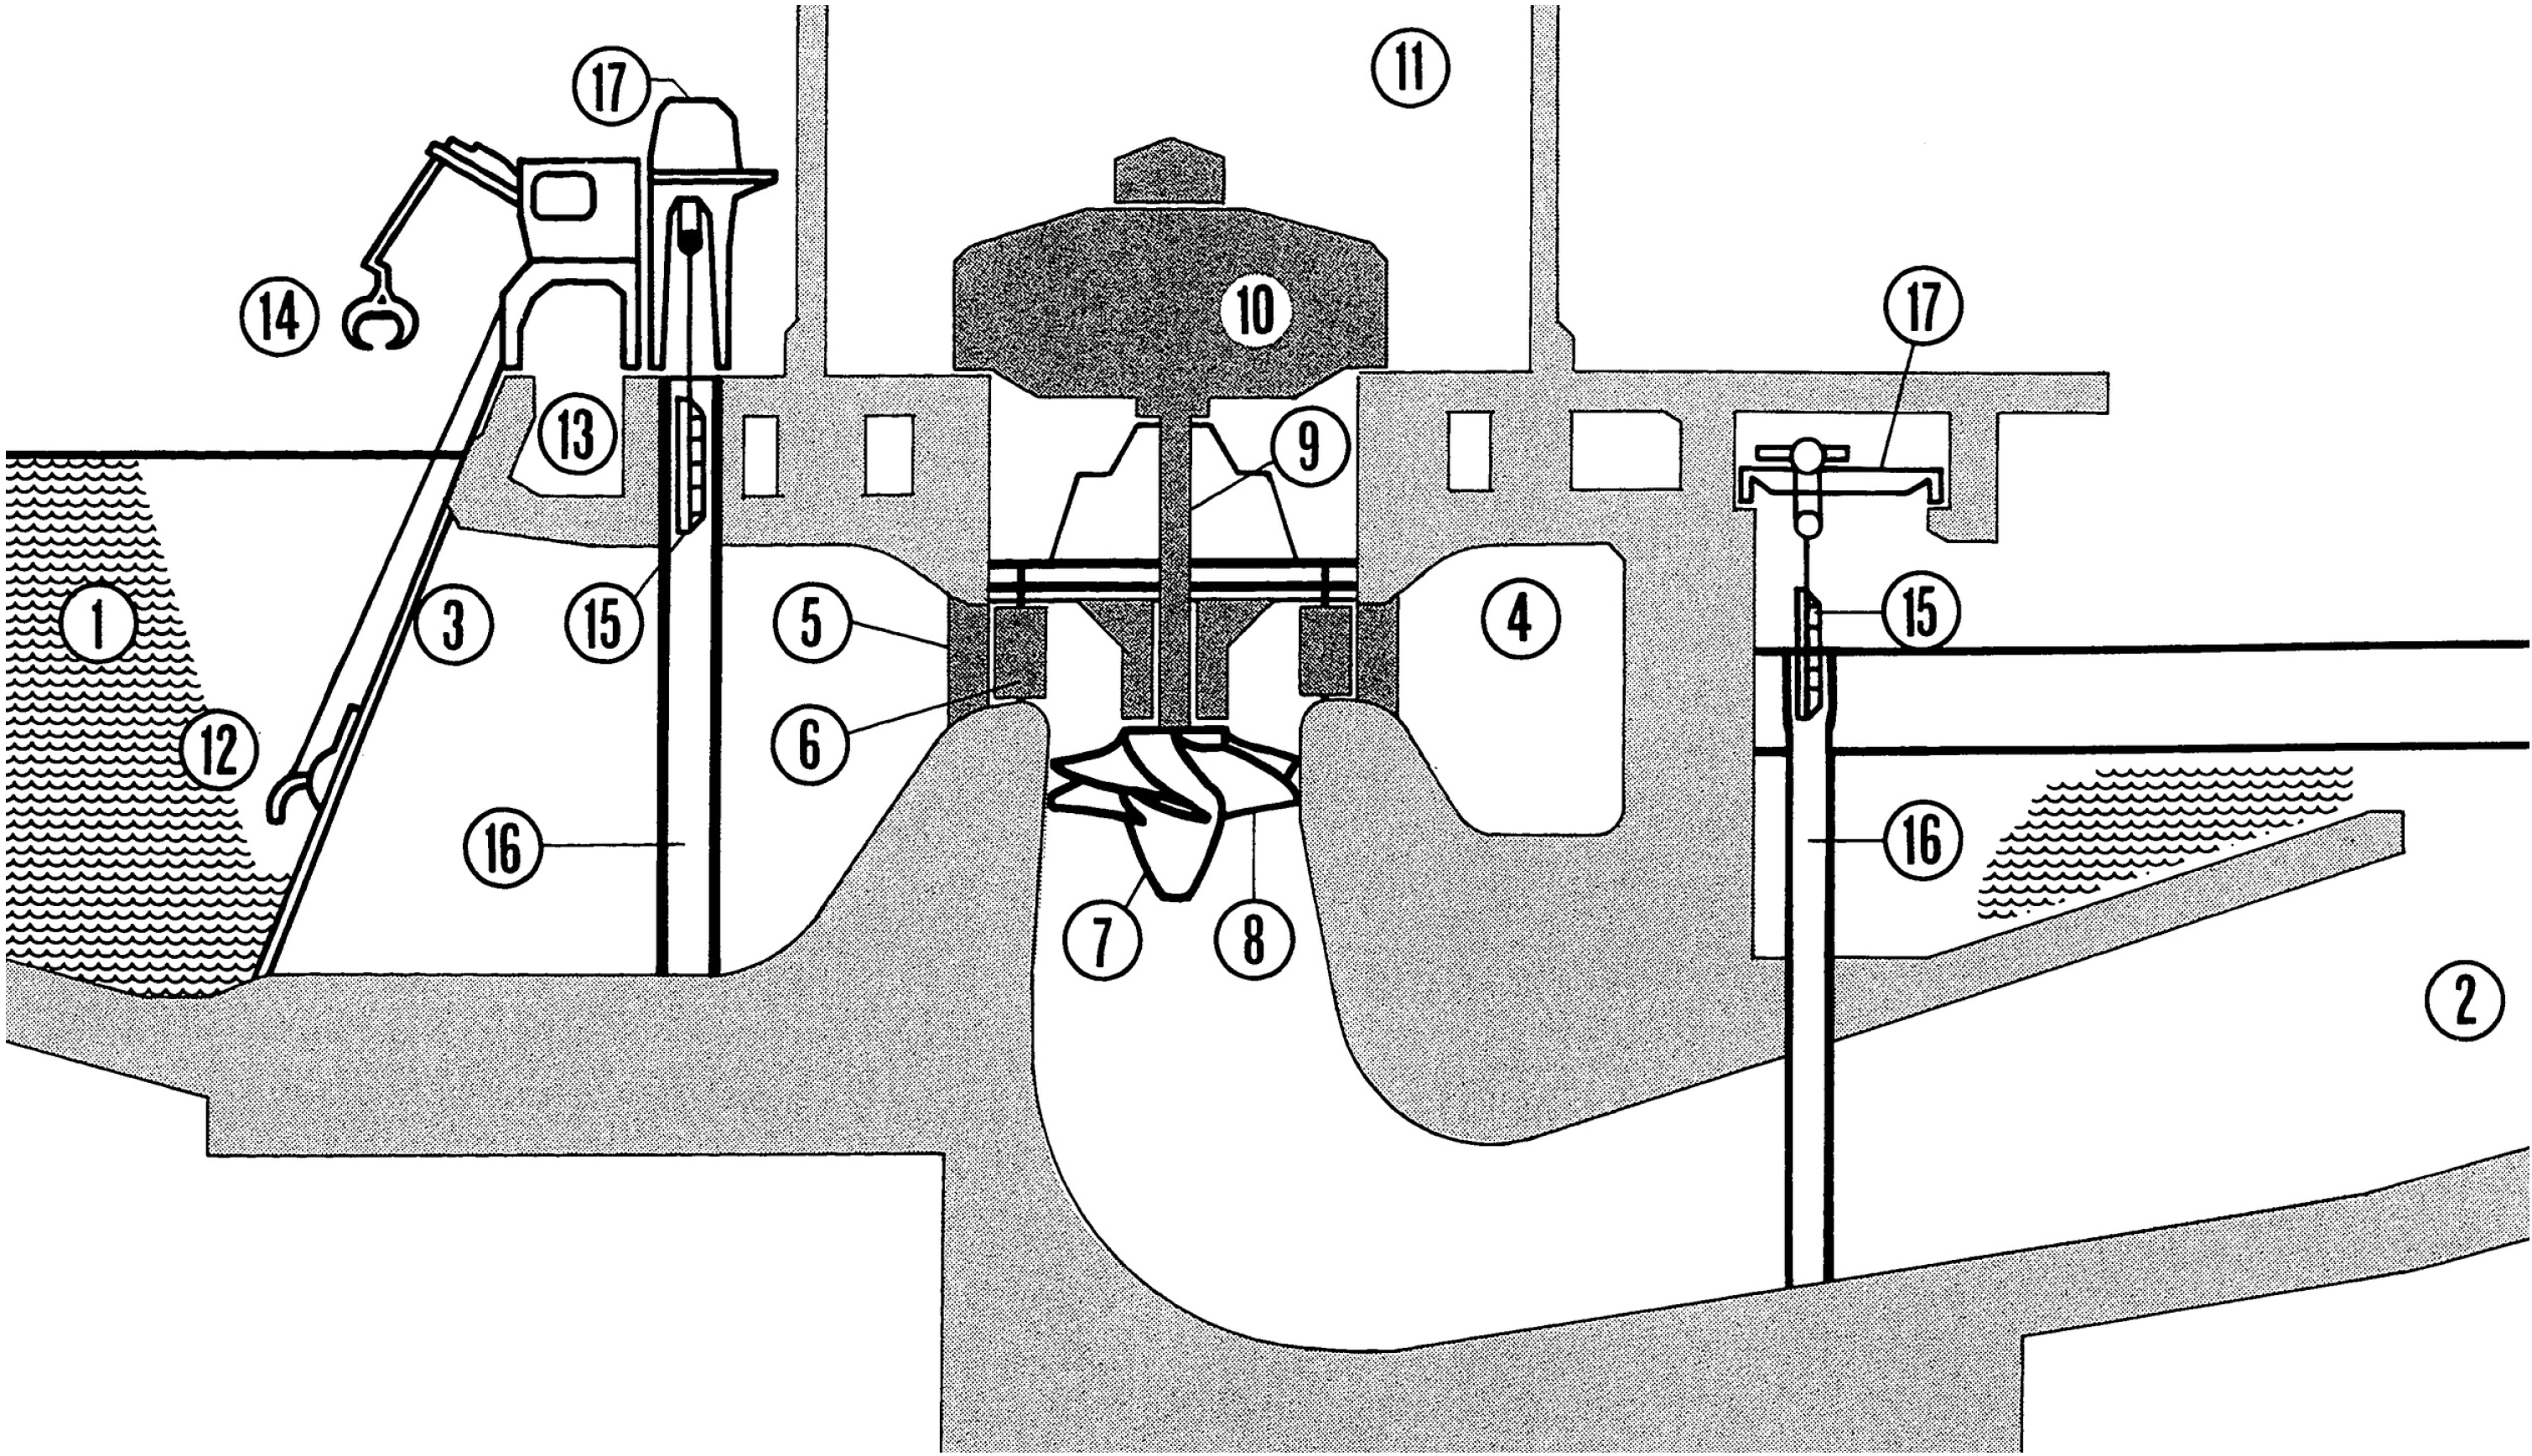
\includegraphics[width=0.75\columnwidth]{images/Laufwasserkraftwerke_Kaplanturbine_Vertikal.png}
    \end{center}

    \vspace{-4mm}
    \def\columnseprulecolor{\color{white}}
    \begin{multicols}{3}
        \begin{enumerate}
            \item Oberwasser
            \item Unterwasser
            \item Rechen
            \item Spirale
            \item Stützschaufeln
            \item Leitschaufeln
            \item Laufrad
            \item Laufradschaufeln
            \item Saugrohr
            \item Generator
            \item Maschinenhaus
            \item Rechenreinigungsmaschine
            \item Geschwemmselrinne
            \item Zangengreifer
            \item Dammbalken
            \item Nuten für Dammbalken
            \item Dammbalkenkran
        \end{enumerate}
    \end{multicols}
    \def\columnseprulecolor{\color{black}}

\subsection{LWK mit Rohrturbinen (horizontal, bis 25m Fallhöhe)}
    \begin{center}
        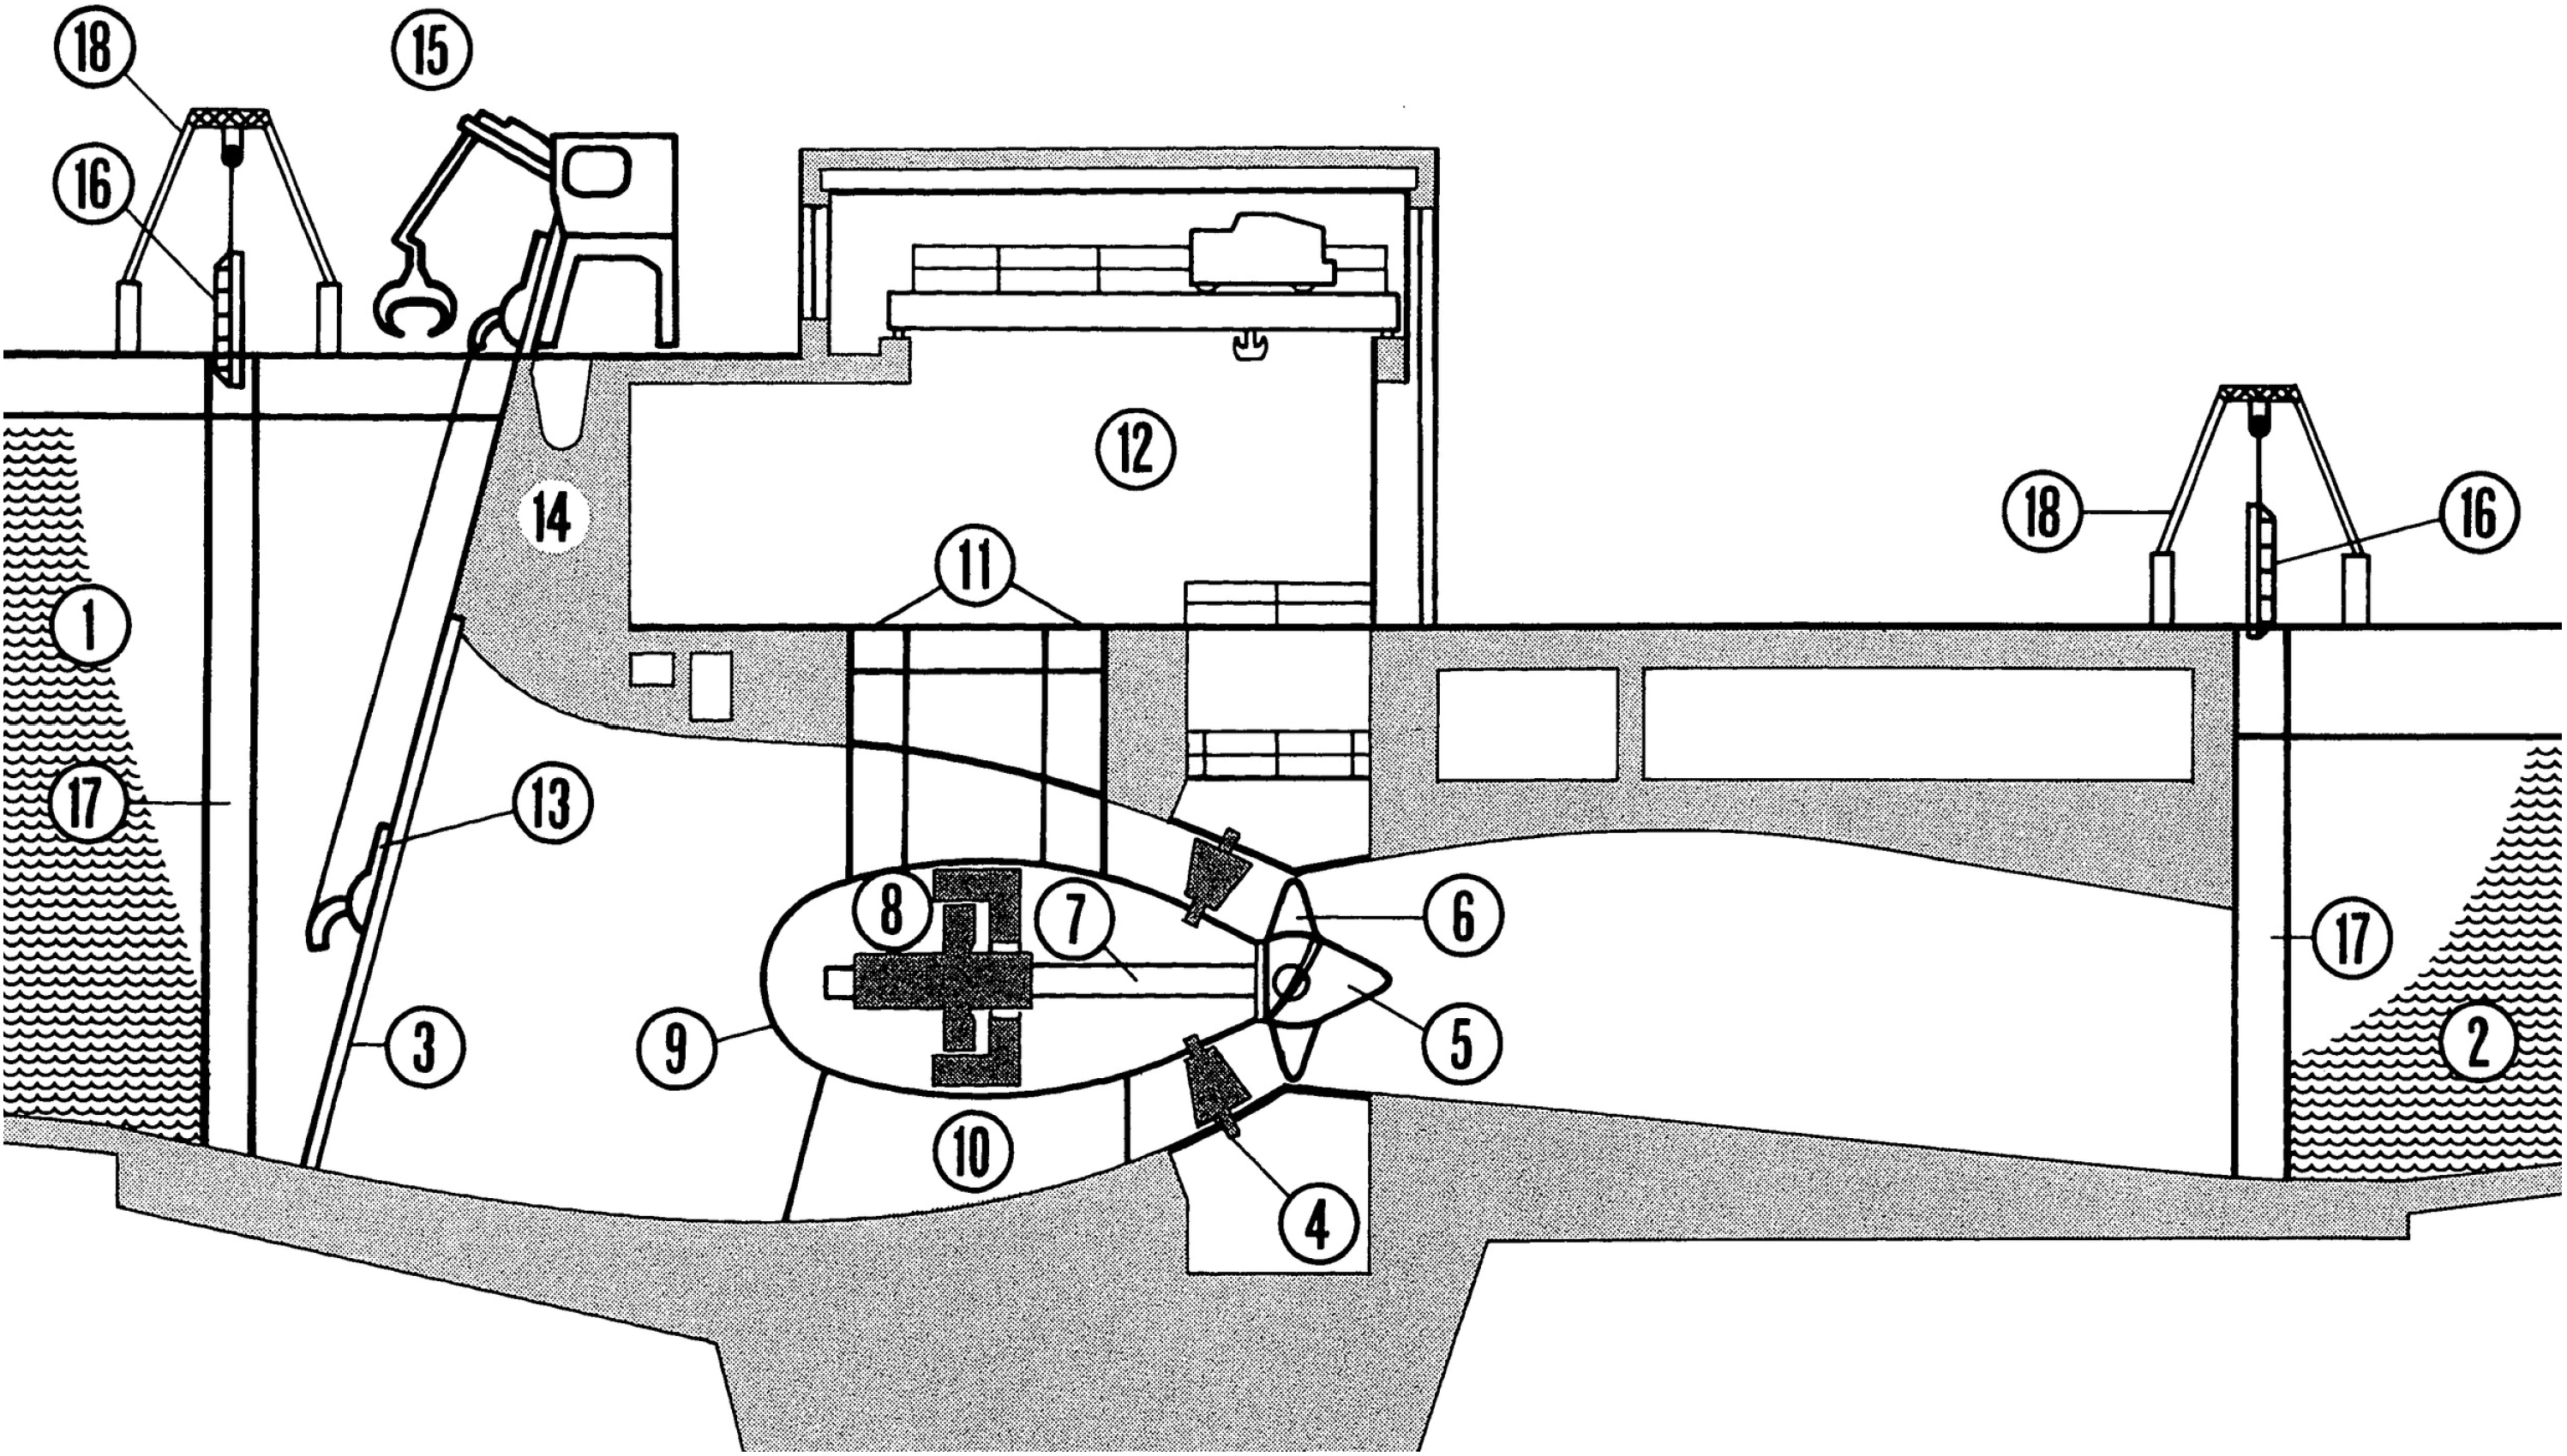
\includegraphics[width=0.9\columnwidth]{images/Laufwasserkraftwerke_Kaplanturbine_Horizontal.png}
    \end{center}

    \vspace{-4mm}
    \def\columnseprulecolor{\color{white}}
    \begin{multicols}{3}
        \begin{enumerate}
            \item Oberwasser
            \item Unterwasser
            \item Rechen
            \item Leitschaufeln
            \item Laufrad
            \item Laufradschaufeln
            \item Turbinenwelle
            \item Generator
            \item Gehäuse
            \item Sockel
            \item Einstiegsschächte
            \item Maschinenhalle
            \item Rechenreinigungsmasch.
            \item Geschwemmselrinne
            \item Zangengreifer
            \item Dammbalken
            \item Nuten für Dammbalken
            \item Dammbalkenkran
        \end{enumerate}
    \end{multicols}
    \def\columnseprulecolor{\color{black}}

\subsection{Wasserwirbelkraftwerk}
    \begin{minipage}[c]{0.58\columnwidth}
        \begin{itemize}
        \item Für Kleinwasserkraft
        \item Geringe Fallhöhen und Durchfluss möglich:\\
        $h \geqq 0.5\text{m}$ und $Q \geqq 0.5 \frac{\text{m}^3}{\text{s}}$
        \item Geringerer Wirkungsgrad
        \item Besser Fischgängig
    \end{itemize}
    \end{minipage}
    \hfill
    \begin{minipage}[c]{0.38\columnwidth}
        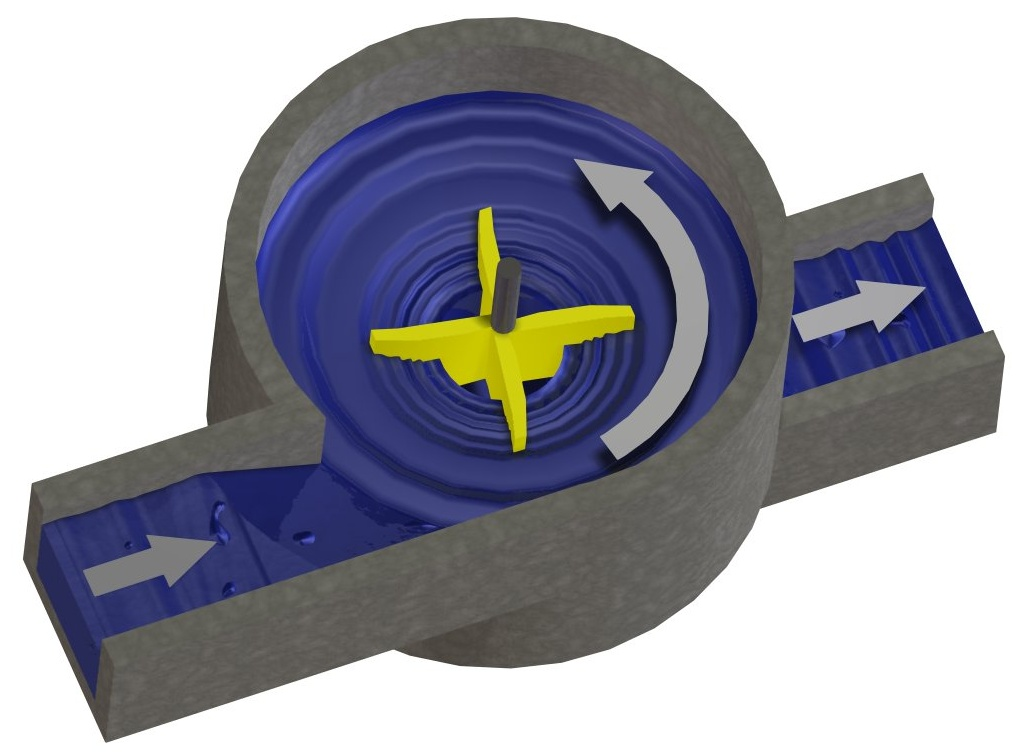
\includegraphics[width=0.65\columnwidth]{images/Wasserwirbelkraftwerk.jpg}
    \end{minipage}

\subsection{LWK mit Strafloturbinen}
    \begin{minipage}[c]{0.7\columnwidth}
        \begin{center}
            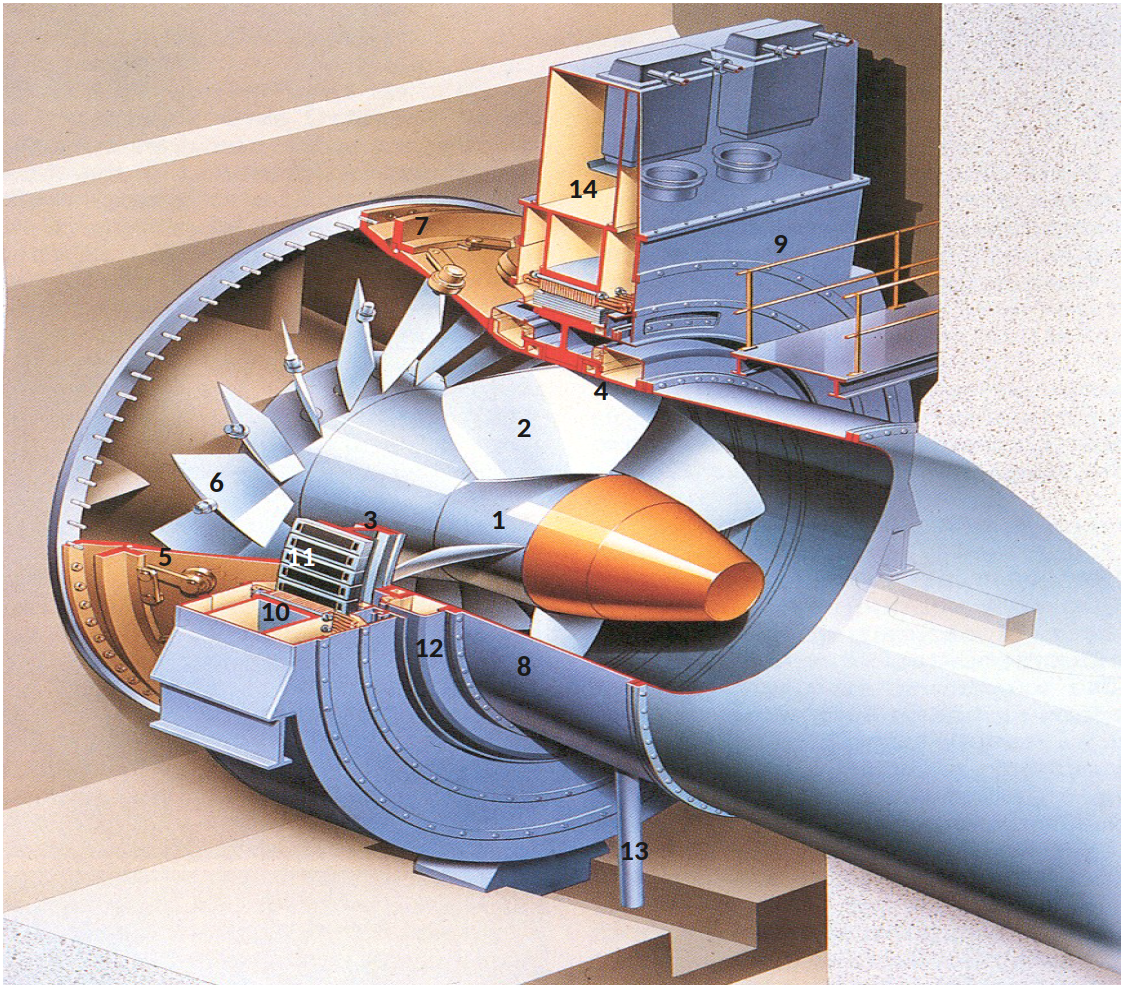
\includegraphics[width=0.95\columnwidth]{images/Laufwasserkraftwerke_mit_Strafloturbinen.png}
        \end{center}
    \end{minipage}
    \hfill
    \begin{minipage}[c]{0.29\columnwidth}
        \begin{enumerate}
            \item Laufradnabe
            \item Propellerblatt
            \item Rotorring
            \item Entlastungsring
            \item Turbinengehäuse
            \item Leitschaufel
            \item Leitradverstellring
            \item Rohrleitung
            \item Generator
            \item Stator
            \item Rotor
            \item Ringdichtungs-Leck"-wasser-Kollektor
            \item Leckwasserableitung
            \item Kühler
        \end{enumerate}
    \end{minipage}

    Weiterentwicklung der Rohrturbine, Rotor Turbine und Generator bilden Einheit

\subsection{Mitteldruckanlagen}
    bis circa 50m Fallhöhe (<= 5 bar Druck)

\subsection{Pumpspeicherkraftwerke (PSW)}
    \begin{minipage}[c]{0.7\columnwidth}
        \begin{center}
            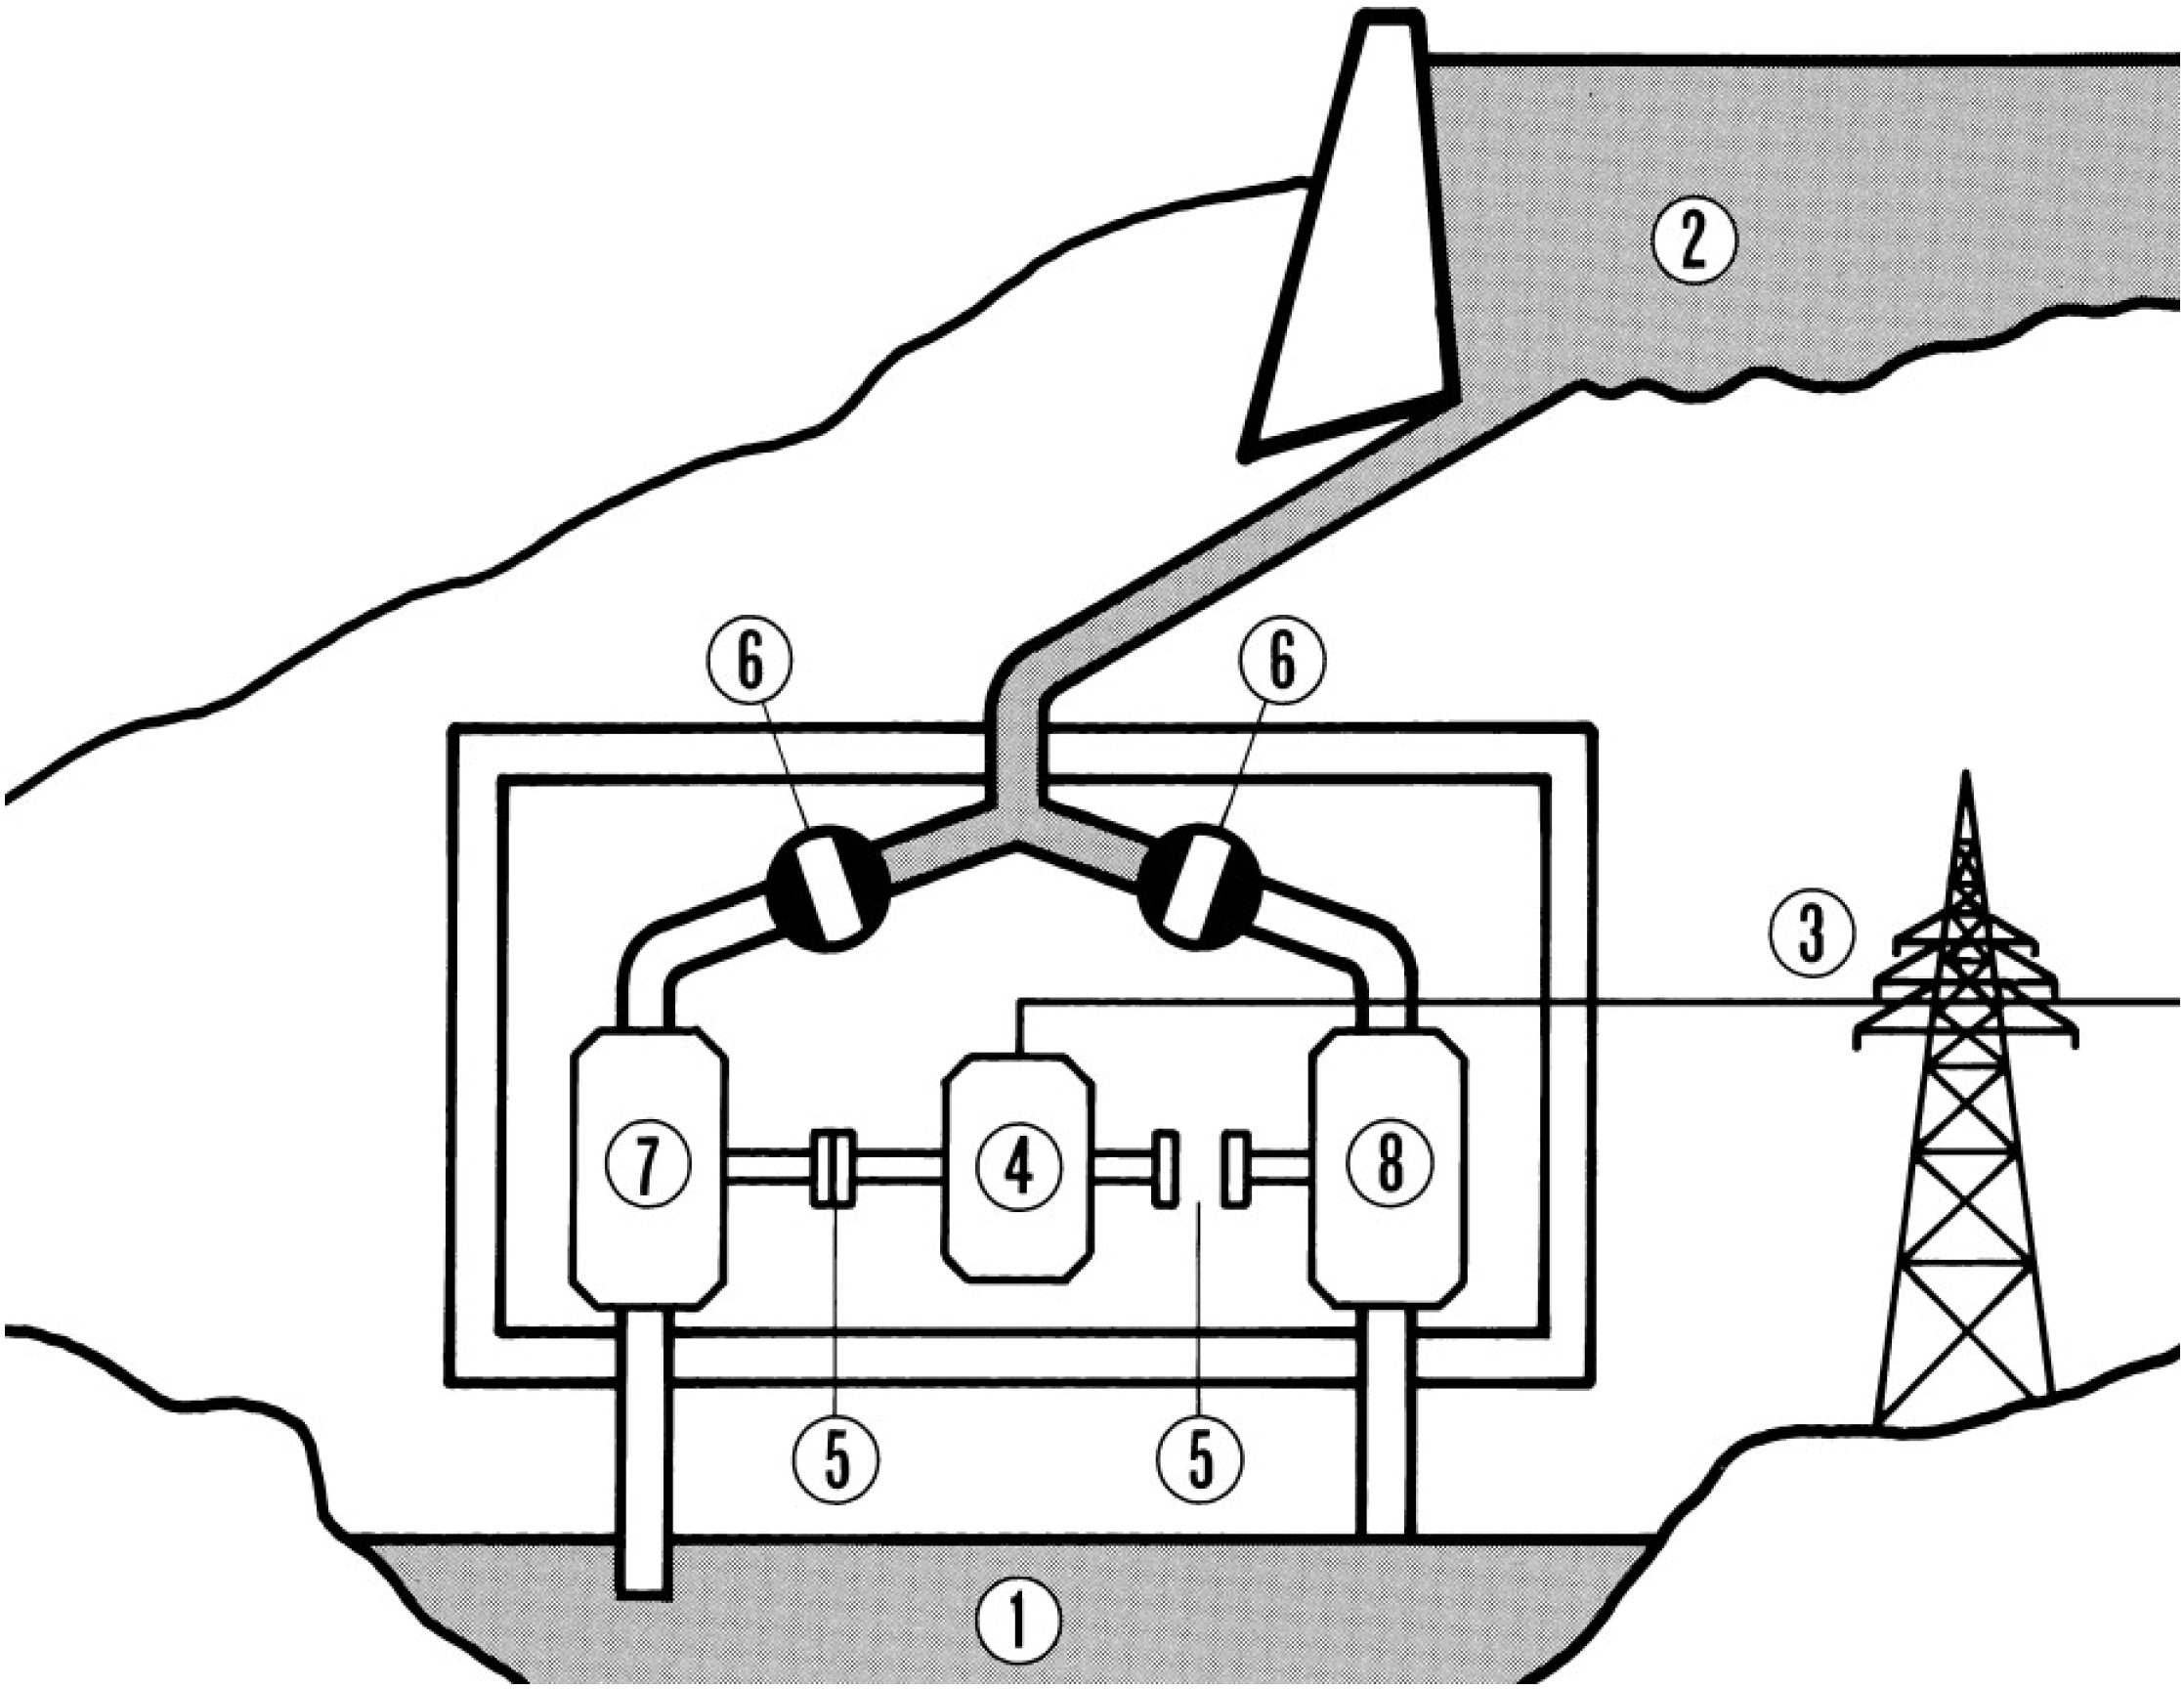
\includegraphics[width=0.95\columnwidth]{images/Pumpspeicherkraftwerke.png}
        \end{center}
    \end{minipage}
    \hfill
    \begin{minipage}[c]{0.29\columnwidth}
        \begin{enumerate}
            \item Unteres Becken
            \item Oberes Becken
            \item Energieableitung, Stromleitung
            \item Motorgenerator
            \item Kupplung
            \item Kugelschieber
            \item Pumpe
            \item Turbine
        \end{enumerate}
    \end{minipage}

    Wirkungsgrad der PSW: 65 – 80\%

\subsubsection{Maschinensatz}
    \begin{tabular}{c c}
        Zweimaschinensatz:  & Motor/Generator und Pumpturbine \\
        Dreimaschinenesatz: & Motor/Generator, Turbine und Pumpe
    \end{tabular}

\subsection{Hochdruck- (Speicher-) Anlagen}
    \begin{minipage}[c]{0.6\columnwidth}
        \begin{center}
            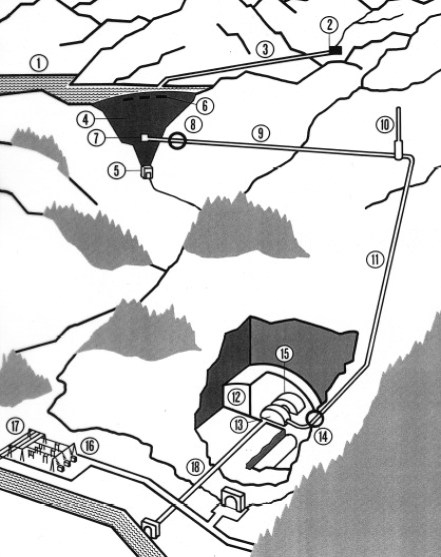
\includegraphics[width=0.95\columnwidth]{images/Hochdruckspeicheranlagen.png}
        \end{center}
    \end{minipage}
    \hfill
    \begin{minipage}[c]{0.39\columnwidth}
        \begin{enumerate}
            \item Stausee
            \item Wasserfassung
            \item Freispiegelstollen 
            \item[] (keine Druckleitung)
            \item Staumauer
            \item Grundablass (für kontr. Ablauf)
            \item Hochwasserentlastung (Überlauf)
            \item Einlauf
            \item Drosselklappe (Wasserfluss Druckstollen steuern)
            \item Druckstollen
            \item Wasserschloss (Druckausgleich Änderung Wasserdurchfluss)
            \item Druckschacht
            \item Zentrale
            \item Turbine
            \item Kugelschieber
            \item Generator
            \item Energieableitung, Transformatoren
            \item Schaltanlage
            \item Unterwasserstollen
        \end{enumerate}
    \end{minipage}

    ab circa 50m Fallhöhe (> 5 bar Druck, bis weit über 100 bar möglich)

\subsubsection{Stollen und Schächte}
    \begin{tabular}{ll}
        Freispiegelstollen:         & flach, nicht voll gefüllt, Umgebungsdruck\\
        Druckstollen (Betonverkl.): & flach, voll gefüllt, Druck $>$ Umgebungsdr. , $v < 5\,\mathrm{m/s}$ \\
        Druckschacht (Stahlpanz.):  & steil, voll gefüllt, Druck $\gg$ Umgebungsdr. , $v < 9\,\mathrm{m/s}$ 
    \end{tabular}

\subsection{Wasserschloss}
    Das Wasserschloss ist ein nach oben offenes Gefäss.
    Im Druckstollen sind grosse Wassermassen vorhanden. Diese Wassermassen müssen:

    \begin{itemize}
        \item beim Anfahren der Maschinengruppen beschleunigt,
        \item beim Abstellen gebremst werden.
    \end{itemize}
    Das Wasserschloss dient als Puffer

    \begin{center}
        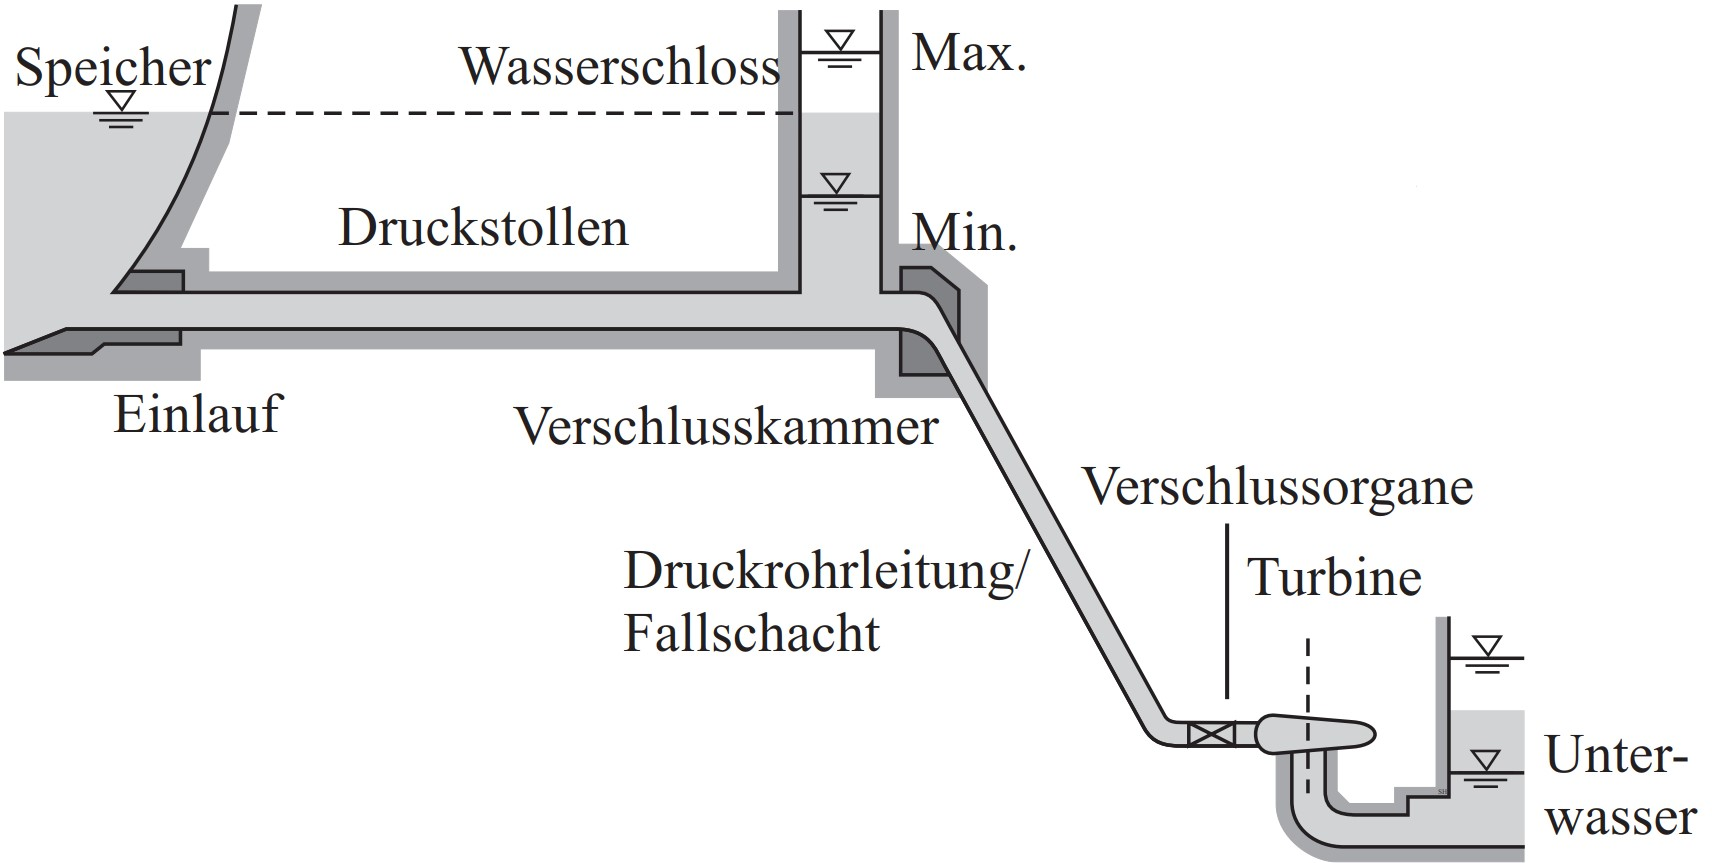
\includegraphics[width=0.6\columnwidth]{images/Wasserschloss.jpg}
    \end{center}

    \begin{minipage}[t]{0.33\columnwidth}
        \subsubsection{Generell}
        $
        \boxed{E_{\mathrm{ktot}} = E_{\mathrm{kSt}}+E_{\mathrm{ks}}} \\
        \boxed{E_{\mathrm{pot}} = E_{\mathrm{ktot}}} \\
        \boxed{h_{\mathrm{ws}} = \sqrt{\frac{E_{\mathrm{pot}} \cdot 2}{\rho_{\mathrm{w}} \cdot A_{\mathrm{ws}} \cdot g}}}
        $
    \end{minipage}%
    \hfill
    \begin{minipage}[t]{0.33\columnwidth}
        \subsubsection{Stollen}
        $
        \boxed{V_{\mathrm{St}} = l_{\mathrm{St}} \cdot A_{\mathrm{St}}}  \\
        \boxed{m_{\mathrm{wSt}} = \rho_{\mathrm{w}} \cdot V_{\mathrm{St}}} \\
        \boxed{v_{\mathrm{St}}= \frac{Q}{A_{\mathrm{St}}}} \\
        \boxed{E_{\mathrm{kSt}} = \frac{m_{\mathrm{wSt}} \cdot v_{\mathrm{St}}^2}{2}}
        $
    \end{minipage}%
    \hfill
    \begin{minipage}[t]{0.33\columnwidth}
        \subsubsection{Schacht}
        $
        \boxed{V_{\mathrm{s}} = l_{\mathrm{s}} \cdot A_{\mathrm{s}}} \\
        \boxed{m_{\mathrm{ws}} = \rho_{\mathrm{w}} \cdot V_{\mathrm{s}}} \\
        \boxed{v_{\mathrm{s}}= \frac{Q}{A_{\mathrm{s}}}} \\
        \boxed{E_{\mathrm{ks}} = \frac{m_{\mathrm{ws}} \cdot v_{\mathrm{s}}^2}{2}}
        $
    \end{minipage}

    \renewcommand{\arraystretch}{1.2}
    \begin{tabular}{@{} l p{7cm} l @{}}    
        $[A_{\mathrm{s}}]$      & Schachtfläche \dotfill                                        & $\mathrm{m^2}$ \\
        $[A_{\mathrm{St}}]$     & Stollenfläche \dotfill                                        & $\mathrm{m^2}$ \\
        $[A_{\mathrm{ws}}]$     & Wasserschlossfläche \dotfill                                  & $\mathrm{m^2}$ \\
        $[g]$                   & Fallbeschleunigung $(9.81\, \mathrm{m/s^2})$ \dotfill         & $\mathrm{m^2}$ \\
        $[h_{\mathrm{ws}}]$     & Höhe des Wasserspiegels im Wasserschloss \dotfill             & $\mathrm{m^2}$ \\
        $[l_{\mathrm{s}}]$      & Schachtlänge \dotfill                                         & $\mathrm{m}$ \\
        $[l_{\mathrm{St}}]$     & Stollenlänge \dotfill                                         & $\mathrm{m}$ \\
        $[m_{\mathrm{ws}}]$     & Wassermasse im Schacht \dotfill                               & $\mathrm{kg}$ \\
        $[m_{\mathrm{wSt}}]$    & Wassermasse im Stollen \dotfill                               & $\mathrm{kg}$ \\
        $[Q]$                   & Druchfluss \dotfill                                           &$\mathrm{m^3/s}$\\
        $[\rho_{\mathrm{w}}]$   & Dichte des Wassers ($1000\, \mathrm{kg/m^3}$) \dotfill        & $\mathrm{kg/m^3}$ \\
        $[V_{\mathrm{s}}]$      & Schachtvolumen \dotfill                                       & $\mathrm{m^3}$ \\
        $[V_{\mathrm{St}}]$     & Stollenvolumen \dotfill                                       & $\mathrm{m^3}$ \\
        $[v_{\mathrm{s}}]$      & Fliessgeschwindigkeit im Schacht\dotfill                      & $\mathrm{m/s}$ \\
        $[v_{\mathrm{St}}]$     & Fliessgeschwindigkeit im Stollen \dotfill                     & $\mathrm{m/s}$ \\
        $[E_{\mathrm{ks}}]$     & Kinetische Energie im Schacht \dotfill                        & $\mathrm{J}$\\
        $[E_{\mathrm{kSt}}]$    & Kinetische Energie im Stollen \dotfill                        & $\mathrm{J}$\\
        $[E_{\mathrm{pot}}]$    & Potentielle Energie           \dotfill                        & $\mathrm{J}$\\
    \end{tabular}
    \newcolumn

\subsection{Gezeitenkraftwerke}
    \begin{itemize}
        \item Nutzung des Tidenhubs
        \item Früher meist mit Staudammbauweise (hohe Umwelteinwirkungen)
        \item Heute meist Meeresströmungs-Kraftwerk
        \item Grösste Europäische Anlage in Frankreich (240 MW)
    \end{itemize}


\subsection{Wellenkraftwerk}
    \subsubsection{Wellenkraftwerk mit Pneumatischer Kammer}
    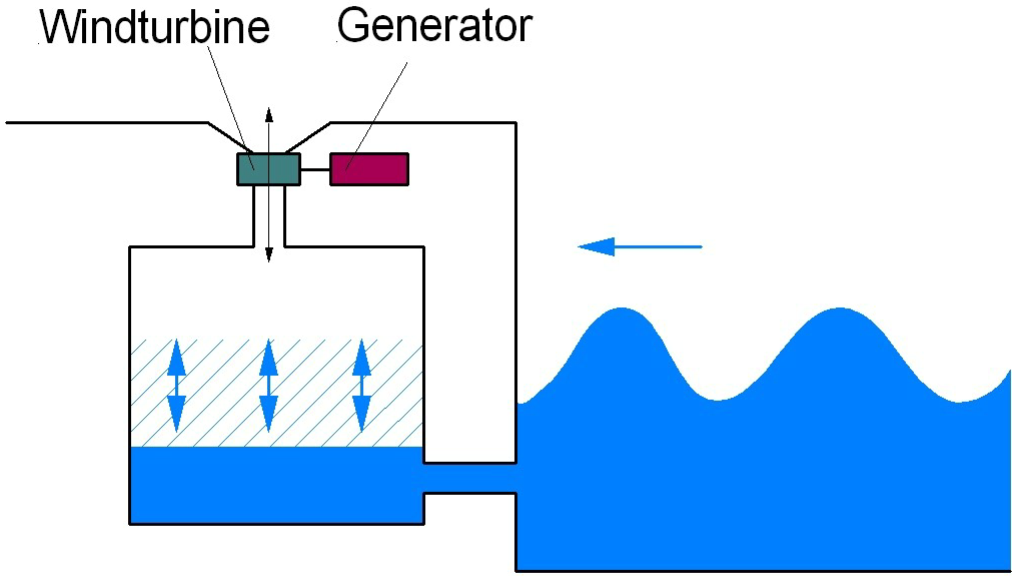
\includegraphics[width=0.55\columnwidth]{images/Wellenkraft mit Pneumatischer Kammer.png}

    \subsubsection{Wellenkraftwerk mit Rampe}
    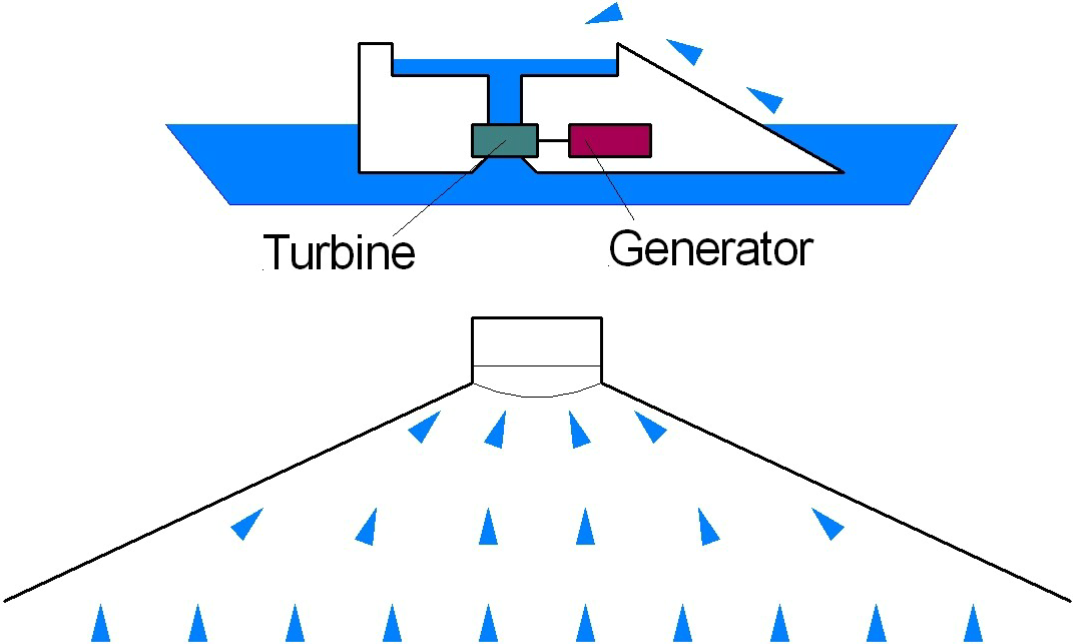
\includegraphics[width=0.55\columnwidth]{images/Wellenkraft mit Rampe.png}